\documentclass[11pt, a4paper]{report}
%--------------Importación de paquetes (preámbulo)--------------%
\input{preambulo}
\usepackage[pdftex,
            pdfauthor={Joseph Jaramillo},
            pdftitle={Informe reporte sísmico},
            pdfsubject={UTN},
            pdfkeywords={Computer UNIVAC Evolutionary},
            pdfproducer={TeXLive},
            pdfcreator={pdflatex, or other tool},
            colorlinks=true,
            linkcolor=black]{hyperref}


%---------------------------------------------------------------%
\graphicspath{ {Figures/} }
\setlength{\parindent}{0em}
\topmargin=0.5cm
\usepackage[lmargin=2cm,rmargin=2cm,bottom=1cm]{geometry}
%%%%%% --- generando caja de pagina como background
\DefineNamedColor{named}{Cyan}{cmyk}{250,250,250,250}
\backgroundsetup{
scale=1,
angle=0,
color=Cyan,
opacity=0.15,
contents={ %\transparent{0.4}

\includegraphics[width=100mm]{Logos/logo_cismid.png}  
%\begin{tikzpicture}[overlay,remember picture]
%\draw [line width=1.5pt]
%    ($ (current page.north west) + (1.0cm,-1.0cm) $) % izquierda, arriba
%    rectangle
%    ($ (current page.south east) + (-1.0cm,0.8 cm) $);  % derecha,abajo
%\draw [line width=1.25pt]
%    ($ (current page.north west) + (1.15cm,-1.15cm) $)
%    rectangle
%    ($ (current page.south east) + (-1.15cm,0.95cm) $); 
%\end{tikzpicture}
}
}

%---------------------------------------------------------------%
\title{CENTRO DE MONITOREO SÍSMICO DEL CISMID-FIC-UNI \\
RED NACIONAL DE ACELERÓGRAFOS (REDACIS)\\
INFORME PRELIMINAR\\
}

%%  -------Encabezado -------%%%
\lhead{\vspace{-1cm} \begin{picture}(0,0) \put(0,0){
\includegraphics[width=18mm]{Logos/logo_uni}} \end{picture}}
\rhead{\vspace{-1cm} \begin{picture}(0,0) \put(-70,0){
\includegraphics[width=27mm]{Logos/logo_cismid}} \end{picture}}
\chead{\vspace{-0.5cm} UNIVERSIDAD NACIONAL DE INGENIERÍA\\
FACULTAD DE INGENIERÍA CIVIL\\
CENTRO PERUANO JAPONÉS DE INVESTIGACIONES\\
SÍSMICAS Y MITIGACIÓN DE DESASTRES\\
\vspace{-0.5cm} }


\renewcommand{\headrulewidth}{1pt}
\renewcommand{\headrule}{\hbox to\headwidth{\color{Cyan}\leaders\hrule height \headrulewidth\hfill}}
\renewcommand{\footrulewidth}{1pt}
\renewcommand{\footrule}{{\color{Cyan}\vskip-\footruleskip\vskip-\footrulewidth \hrule width\headwidth height\footrulewidth\vskip\footruleskip}}
%\futurelet\TMPfootrule\def\footrule{{\color{blue}\TMPfootrule}}
\setlength\headheight{40.0pt}
\addtolength{\textheight}{-100.0pt}
\cfoot{\scriptsize AV. TÚPAC AMARU N° 1150 – LIMA 25 – PERÚ – Apartado Postal 31-250 Lima 31\\
		Teléfono (511)482-0777, (511)482-0804, (511)482-0790   Fax: (511)481-0170 \\
		e-mail: director@uni.edu.pe   http://www.cismid.uni.edu.pe
		}

\pagestyle{fancy}

%%%%%
%-------------------CUERPO-------------------%
\begin{document}
%\listoffigures

%\listoftables

%\newpage


\begin{pycode}
from Python_tools.core import Event
import pandas as pd

event = Event.load_event_properties('D:/SHM/code-jj/Report/Event.sav')

lugar = event.epicenter["Place"].iloc[0]
fecha = event.epicenter["Date"].iloc[0]
hora_local = event.epicenter["Local Hour"].iloc[0]
hora_UTC = event.epicenter["UTC Hour"].iloc[0]
referencia = event.epicenter["Venue"].iloc[0]
institucion = event.epicenter["Institution"].iloc[0]
latitud = event.epicenter["Latitude"].iloc[0]
longitud = event.epicenter["Longitude"].iloc[0]
profundidad =  event.epicenter["Depth"].iloc[0]
magnitud = event.epicenter["Magnitude"].iloc[0]
nstations = str(len(event.station)).zfill(2)


print(r'\begin{center}')
print(r'\centering')
print(r'\textbf{CENTRO DE MONITOREO SÍSMICO DEL CISMID-FIC-UNI \\')
print(r'RED DE MONITOREO DE EDIFICACIONES\\}')
print(r'\vspace{0.3cm}')

print(r'\textbf{INFORME PRELIMINAR\\}')
print(r'\vspace{0.3cm}')

print(r'\textbf{Acelerogramas del Sismo de %s del %s}' %(lugar, fecha))
print(r'\vspace{0.25cm}')
print(r'\end{center}')

print(r'El %s a las %s (hora local), ocurrió un sismo con epicentro a %s (Fuente: %s). Las características sísmicas del evento ' %(fecha,hora_local,referencia,institucion) )

\end{pycode}
se resumen en la Tabla (\ref{tab:tab01}) y la ubicación del epicentro, así como de las estaciones 
acelerográficas más cercanas, se muestra en la Figura (\ref{tab:tab01}). \\

\begin{pycode}
print(r'\begin{figure}[H]')
print(r'\begin{multicols}{2}')
print(r'\begin{minipage}[c]{7.5cm}')
print(r'\centering')
print(r'\renewcommand{\arraystretch}{1.8}')
print(r'\captionof{table}{Datos sísmicos (Fuente: %s)} \label{tab:tab01}' %(institucion))
print(r'\begin{tabulary}{7.0cm}{|l|C|}')

print(r'\hline')
print(r'Hora local (UTC-5): & %s \\ \hline' %(hora_local))
print(r'Hora UTC 0: & %s \\ \hline'%(hora_UTC))
print(r'Latitud ($^{\circ}$): & %s \\ \hline'%(latitud))
print(r'Longitud ($^{\circ}$): & %s \\ \hline'%(longitud))
print(r'Profundidad (km): & %s \\ \hline'%(profundidad))
print(r'Magnitud (ML): & %s \\ \hline'%(magnitud))
print(r'Lugar de referencia: & %s. \\ '%(referencia))
print(r'\hline')
print(r'\end{tabulary}')
print(r'\end{minipage}')

print(r'\hspace{0.5cm}')

print(r'\begin{minipage}[c]{8.2cm}')
print(r'\centering %%\captionsetup{format = hang, width=8cm}')
print(r'\setlength\fboxsep{0pt}')
print(r'\setlength\fboxrule{0.3pt}')
print(r'\captionof{figure}{Epicentro y estaciones cercanas.}  \label{fig:fig01}')
print(r'% \begin{figure}')
print(r'\fbox{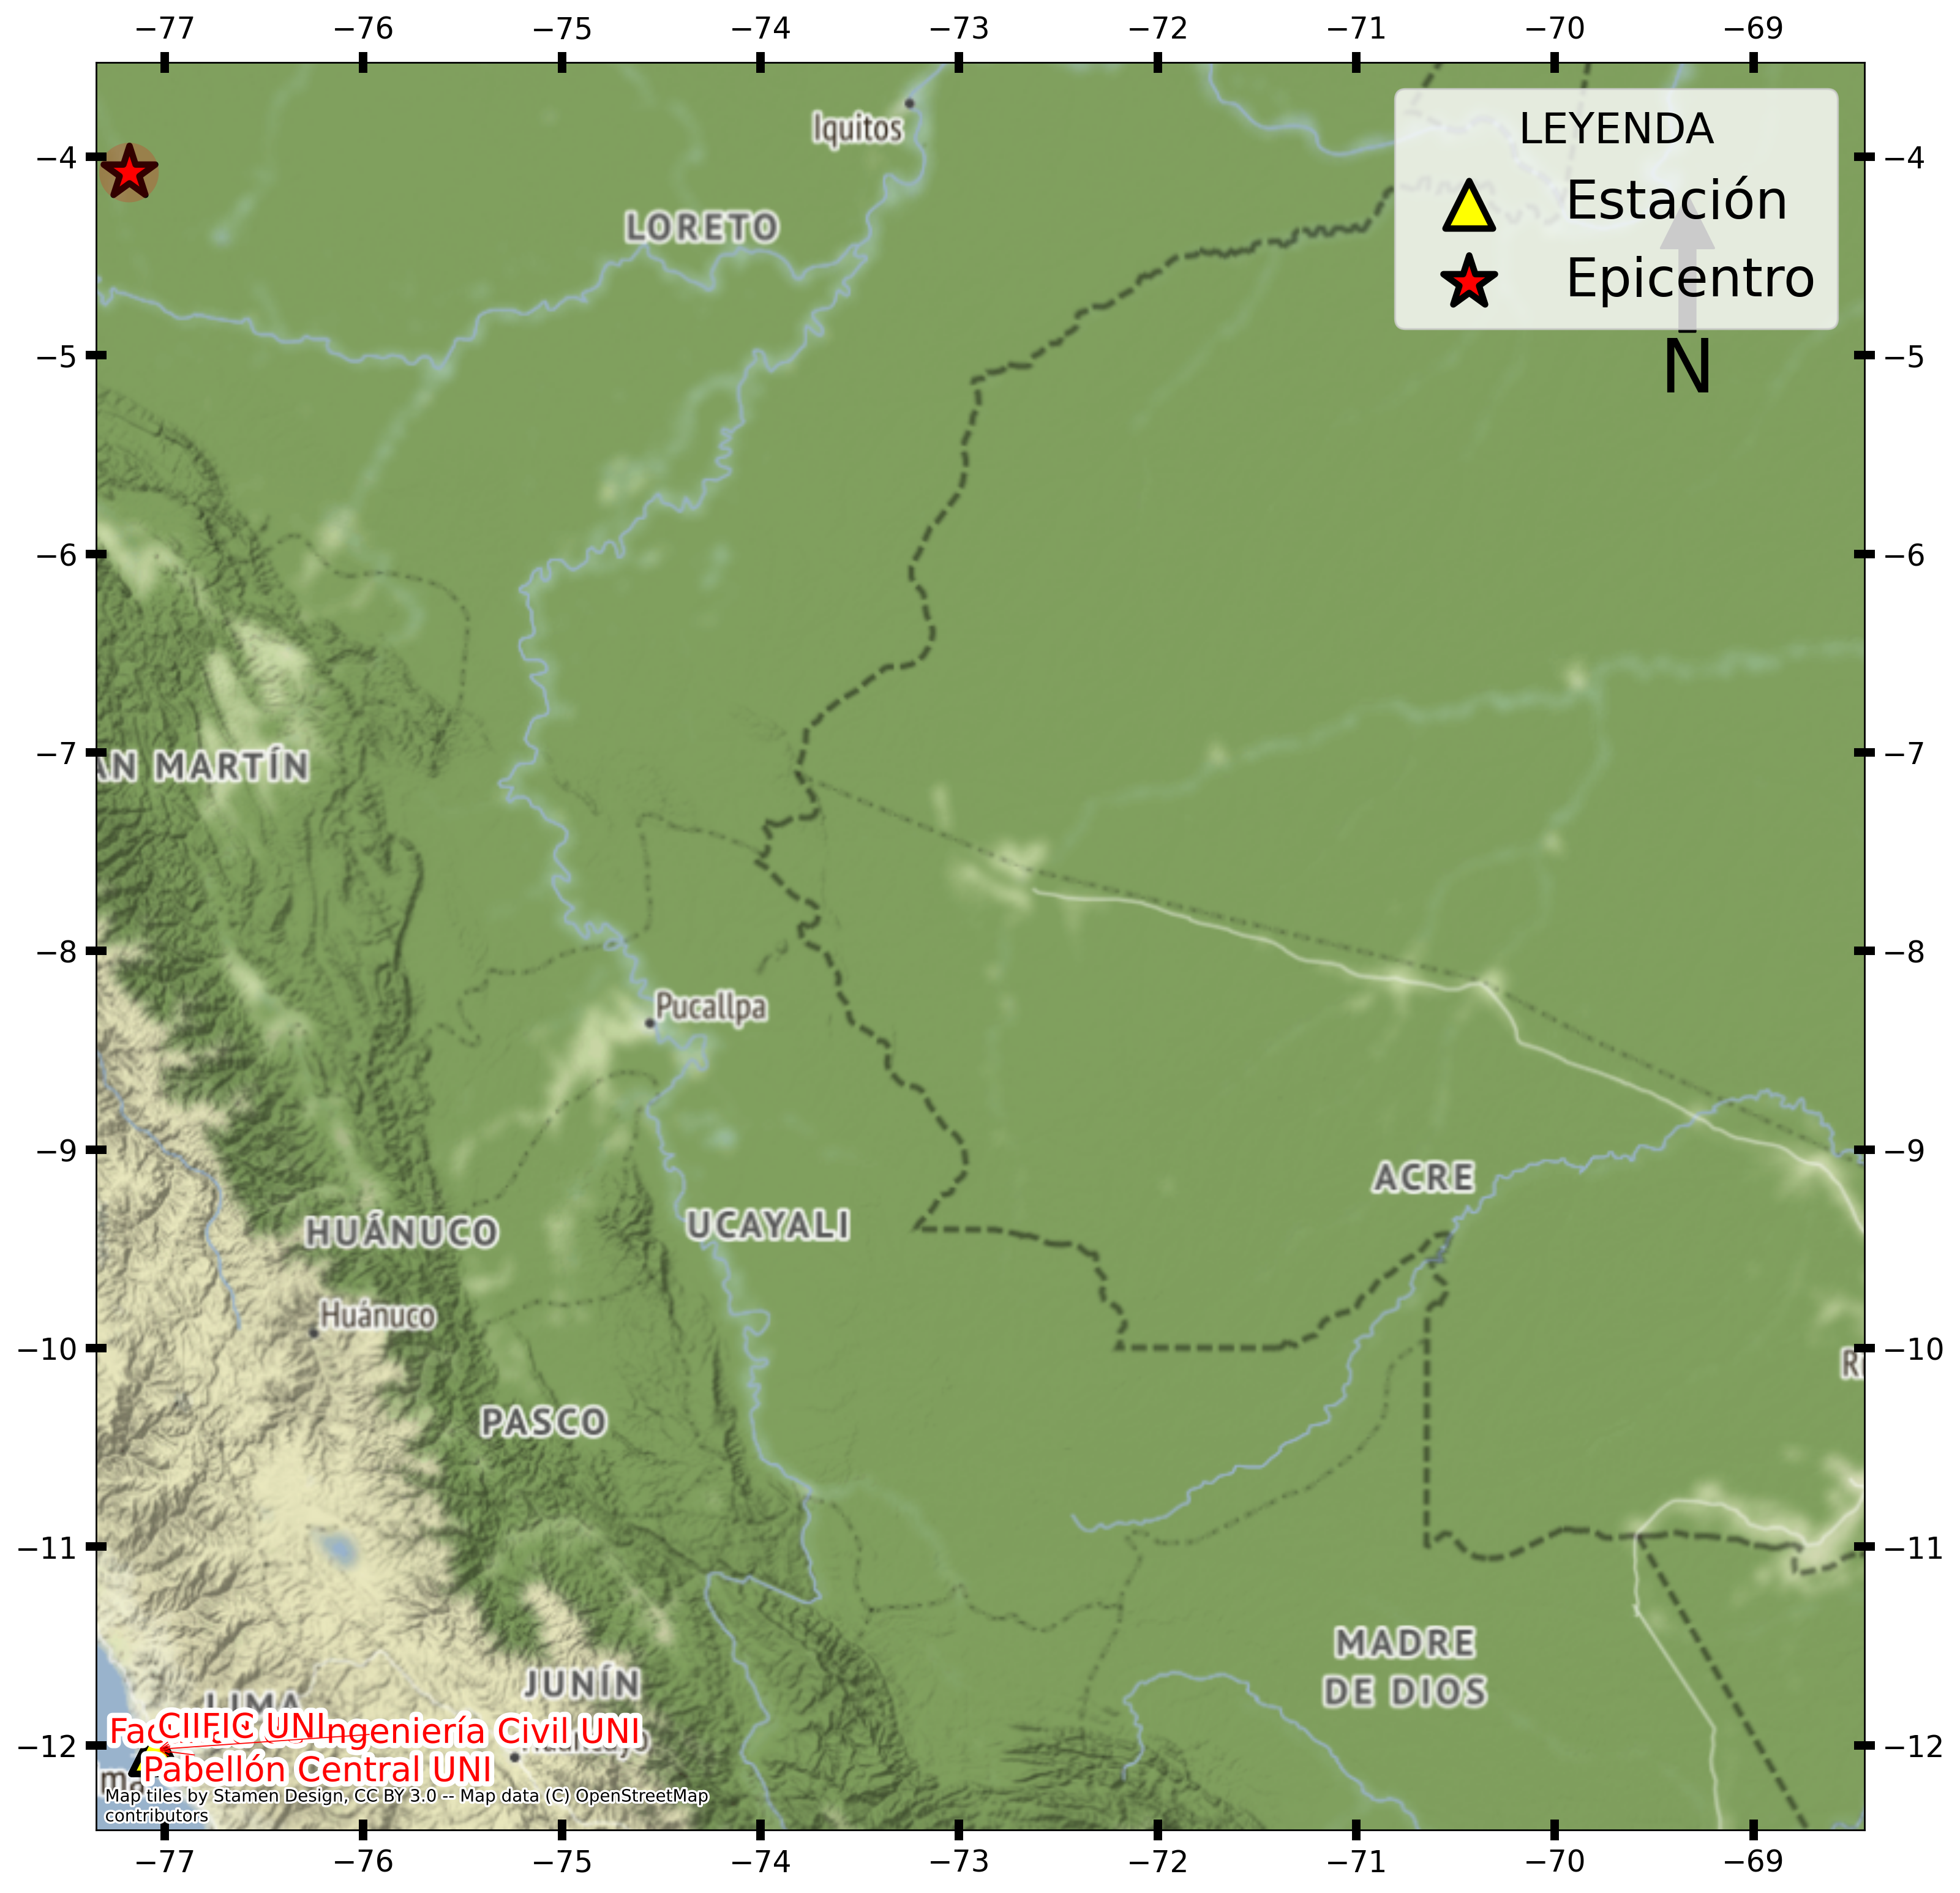
\includegraphics[trim={1mm 0.5mm 1mm 0.5mm},clip,width=1.0\textwidth]{Mapa01.png}}')
print(r'% \end{figure}')
print(r'\end{minipage}')
print(r'\end{multicols} ')
print(r'\end{figure}')

print(r'\vspace{1cm}')

print(r'\noindent')
print(r'En este reporte, la Red de Monitoreo de Edificaciones (REMOED) del Centro Peruano Japonés de Investigaciones Sísmicas y Mitigación')
print(r'de Desastres (CISMID) FIC-UNI presenta de manera preliminar, los registros sísmicos obtenidos de este evento correspondiente a ')
print(r'%s estaciones acelerográficas ubicadas en la ciudad de Lima, cuyos valores de aceleración máxima, para cada '%(nstations))

\end{pycode}
componente, y localizaciónes se muestran en la Tabla (\ref{tab:tab02}) y Figura (\ref{fig:fig02}) respectivamente.\\

\begin{pycode}
pga_max = round(event.max_station["Max_pga"].iloc[0], 2)
direccion = event.max_station["Channel_max_pga"].iloc[0]
stationmax = event.max_station["Id"].iloc[0]
stationmaxubic = event.max_station["Location"].iloc[0]

cap_fig2 = "Aceleraciones máximas registrados en las estaciones acelerográficas ubicadas en la ciudad de Lima correspondientes al sismo de {0} del {1} a las {2} (hora local)".format(lugar, fecha, hora_local)

print(r'\newpage')
print(r'\noindent')
print(r'El máximo valor de PGA registrado en estas estaciones es de %s cm/s2 en la dirección %s ' %(pga_max, direccion))
print(r'correspondiente a la estación %s (%s).'%(stationmax, stationmaxubic))
print(r'Finalmente, en el Anexo adjunto se presentan las gráficas de los acelerogramas obtenidos ')
print(r'en las %s estaciones (direcciones EW, NS y vertical).'%(nstations))

print(r"\renewcommand{\arraystretch}{1.2}")
print(r"\begin{longtable}{|c|c|c|c|}")
print(r"\caption{%s}\label{tab:tab02}\\"%(cap_fig2))
print(r"\hline")
print(r"\textbf{Código} & \textbf{Orientación} & \textbf{Ubicación (Provincia, Departamento)} & \textbf{\begin{tabular}[c]{@{}c@{}}PGA\\ (cm/s2)\end{tabular}} \\ \hline")
# print(r"\hline")
print(r"\endfirsthead")
# print(r"\hline")
# print(r"\textbf{Código} & \textbf{Orientación} & \textbf{Ubicación (Provincia, Departamento)} & \textbf{\begin{tabular}[c]{@{}c@{}}PGA\\ (cm/s2)\end{tabular}} \\ \hline")
# print(r"\hline")
print(r"\endhead")
print(r"\endfoot")
print(r"\endlastfoot")

for i in range(len(event.station)):
    print(r"\multirow{3}{*}{%s}"%(event.station["Id"].iloc[i]),r" & %s & \multirow{3}{*}{\begin{tabulary}{8cm}{@{}C@{}} %s\end{tabulary}}"%(event.station["Channels"].iloc[i][0], event.station["Location"].iloc[i]),r" & %.2f \\ \cline{2-2} \cline{4-4}"%(event.station["PGAs"].iloc[i][0]))
    print(r" & %s &  & %.2f \\ \cline{2-2} \cline{4-4}"%(event.station["Channels"].iloc[i][1], event.station["PGAs"].iloc[i][1]))
    print(r" & %s &  & %.2f \\ \hline"%(event.station["Channels"].iloc[i][2], event.station["PGAs"].iloc[i][2]))
    if (i+1) == 9 or (i-8) % 11 == 0:
        print(r"\pagebreak")
print(r"\end{longtable}")

print(r"\newpage")

print(r'\begin{figure}[!h]')
print(r'\centering')
print(r'\caption{Mapa de ubicación de las estaciones acelerográficas en la ciudad de Lima}')
print(r'\label{fig:fig02}')
print(r' \setlength\fboxsep{0pt}')
print(r'\setlength\fboxrule{0.3pt}')
print(r'\fbox{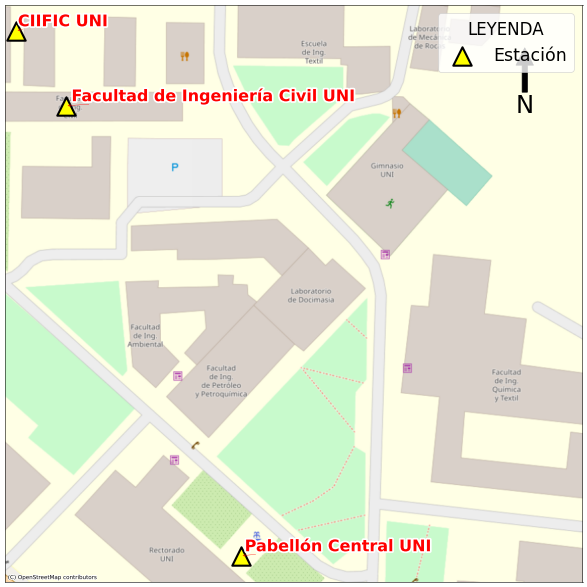
\includegraphics[trim={1mm 1mm 1mm 1mm},clip,width=\textwidth]{Mapa02.png}}')

print(r'\end{figure}')

print(r'\clearpage')

print(r'\vspace*{\fill}% * is needed here')
print(r'\noindent')
print(r'\raisebox{0.5cm}{')
print(r'\makebox[\textwidth]{\hfill {\fontsize{30}{10}\selectfont ANEXO \\ \\ \\ }\hfill }}')
print(r'\raisebox{-0.5cm}{')
print(r'\makebox[\textwidth]{\\ \\ \hfill {\fontsize{24}{20}\selectfont REGISTROS TIEMPO HISTORIA \\  } \hfill }}')
print(r'\vfill')

print(r'\clearpage')

for i in range(event.station.shape[0]):
    channel = event.station.iloc[i]["Channels"]
    fig = event.station.iloc[i]["Graf Acc_Four"]
    for j in range(3):
        capth = 'Registro de Acerelaciones y Espectros de Fourier de la estación %s en dirección %s.' %(event.station["Id"].iloc[i], channel[j])
        print(r'\begin{figure}[!ht]')
        print(r"\caption{%s}"%capth)
        print(r"\label{fig: figura_%s}"%fig[j].split('.')[0])
        print(r"\centering")
        print(r"\includegraphics{%s}"%fig[j].split('.')[0])
        print(r"\end{figure}")
        print(r'\newpage')
print(r"\clearpage")

\end{pycode}

\newpage

\listoffigures

\listoftables

\newpage

\end{document}